\section{Vertically isothermal disks with 
  isothermal perturbations}
The linear problem simplifies considerably for the case
$\Gamma=\gamma=1$. Then 
\begin{align}
  Q=W. 
\end{align}

Inserting this into Eq. \ref{ode_w} gives a single equation for the linear stability
problem for isothermal perturbations in a vertically isothermal disk, 
\begin{align}\label{iso_ode}
  \frac{d^2W}{dz^2} + \left(\frac{d\ln{\rho}}{dz} - \frac{\ii k_x
      r}{D}\frac{d\Omega^2}{dz}\right) \frac{dW}{dz} +
  \sigma^2\left(\frac{1}{c_s^2} + \frac{k_x^2}{D}\right)W=0, 
\end{align} 
subject to appropriate boundary conditions. We remark that Eq
.\ref{iso_ode} is also applicable for    
$\gamma=\Gamma\neq 1$ in the limit $t_c\to\infty$ (i.e. adiabatic
disks with adiabatic vertical stratification), since in that case  
$Q\simeq W$ as well. 


\subsection{Neccessity of vertical shear for instability}\label{integral_relation}
We can establish a neccessary condition for instability with the
following assumptions:

\begin{enumerate}
\item We consider eigenvalues such that
  $|\sigma^2|\ll \kappa^2$. Then we can replace $D=\kappa^2 -\sigma^2\to
  \kappa^2$. The problem simplifies because the eigenvalue now only
  appears in the last term in Eq. \ref{iso_ode}. 
\item We are mainly interested in the effect of vertical shear, i.e. $q\neq
0$. This is already captured explicitly in Eq. \ref{iso_ode} through
the factor $d\Omega^2/dz$. We 
therefore simplify further by ignoring the vertical dependence of
$\kappa^2$. For clarity, we will replace  $\kappa^2$ with $\Omega_k^2$.  
\end{enumerate}

{\bf implicit limit on domain size. cannot be too large, otherwise omega reaches small values. should remain of order
omegak}

With these approximations we can re-write the governing equation as
\begin{align}\label{iso_ode1}
  &\frac{d}{dz}\left(\rho e^{-\ii k_x r
      \Omega^2/\Omega_k^2}\frac{dW}{dz}\right) +
  \sigma^2\left(\frac{1}{c_s^2}+\frac{k_x^2}{\Omega_k^2}\right) \rho W e^{-\ii k_x r
    \Omega^2/\Omega_k^2} \notag\\
  &=0.
\end{align}
Next, we multiply Eq. \ref{iso_ode1} by $W^{*}\exp{\left(\ii k_x r
    \Omega^2/\Omega_k\right)}$ and integrate 
vertically from $z=-\zmax$ to $z=\zmax$. We assume either $W$ or
$dW/dz$ vanishes at $z=\pm \zmax$, or that $\zmax$ is sufficiently
large so that the boundary terms are negligible because of the
decaying background density with increasing height. Then,
\begin{align}\label{neccessary_cond}
   &\sigma^2\left(\frac{1}{c_s^2}+\frac{k_x^2}{\Omega_k^2}\right)\int_{-\zmax}^{\zmax}\rho|W|^2dz \notag\\
  &=\int_{-\zmax}^{\zmax}\rho\left|\frac{dW}{dz}\right|^2dz 
  +\frac{\ii k_x r}{\Omega_k^2}\int_{-\zmax}^{\zmax}\rho\frac{d\Omega^2}{dz}W^*\frac{dW}{dz}dz. 
\end{align}
It follows that for instability ($\imag\sigma>0$), it is neccessary to
have $d\Omega^2/dz\neq 0$, i.e. vertical shear.  

\subsection{Maximum growth rate}   
Here we show that the growth rate is limited by the maximum vertical
shear in the domain. It is convenient to introduce the dimensionless
vertical co-ordinate $\hat{z} = z/\Hiso$ and wavenumber
$\hat{k}=k_x\Hiso$. Then 
the integral relation Eq. \ref{neccessary_cond} becomes 
\begin{align}\label{integral_relation1}
  &\left(\frac{\sigma}{\Omega_k}\right)^2\left(1+\hat{k}^2\right)
  \int_{-z_\mathrm{max}}^{z_\mathrm{max}}\rho|W|^2d\hat{z}  
  \notag\\ 
  &=\int_{-z_\mathrm{max}}^{z_\mathrm{max}}\rho\left|\frac{dW}{d\hat{z}}\right|^2d\hat{z}      
  +\ii
  \epsilon\hat{k}q\int_{-z_\mathrm{max}}^{z_\mathrm{max}}\rho
  f(\hat{z}) W^*\frac{dW}{d\hat{z}}d\hat{z},    
\end{align}   
where $f(\hat{z})$ is defined such that
\begin{align}\label{fz_shear}
  \frac{d\Omega^2}{d\hat{z}} = \epsilon^2q f(\hat{z})\Omega_k^2.
\end{align}

For convenience, we write $\hat{\sigma}\equiv\sigma/\Omega_k = \hat{\omega} +
\ii\hat{\nu}$ with $\hat{\omega},\hat{\nu}$ being the dimensionless
mode frequency and growth rates. Then the real and imaginary parts of
Eq. \ref{integral_relation1} are
\begin{align}
  &\left(\hat{\omega}^2-\hat{\nu}^2\right)\left(1+\hat{k}^2\right)
   \int_{-z_\mathrm{max}}^{z_\mathrm{max}}\rho|W|^2d\hat{z} -
  \int_{-z_\mathrm{max}}^{z_\mathrm{max}}\rho\left|\frac{dW}{d\hat{z}}\right|^2d\hat{z}
  \notag\\
  &=\real\left[\ii
  \epsilon\hat{k}q\int_{-z_\mathrm{max}}^{z_\mathrm{max}}\rho
 f(\hat{z}) W^*\frac{dW}{d\hat{z}}d\hat{z}\right], \notag\\
& 2\hat{\omega}\hat{\nu}\left(1+\hat{k}^2\right)
   \int_{-z_\mathrm{max}}^{z_\mathrm{max}}\rho|W|^2d\hat{z}\notag\\
   &=\imag\left[\ii
  \epsilon\hat{k}q\int_{-z_\mathrm{max}}^{z_\mathrm{max}}\rho
 f(\hat{z}) W^*\frac{dW}{d\hat{z}}d\hat{z}\right].
\end{align}
Adding the square of these equations give
\begin{align}
&\left[|\hat{\sigma}|^2\left(1+\hat{k}^2\right)
   \int_{-z_\mathrm{max}}^{z_\mathrm{max}}\rho|W|^2d\hat{z} -
  \int_{-z_\mathrm{max}}^{z_\mathrm{max}}\rho\left|\frac{dW}{d\hat{z}}\right|^2d\hat{z}\right]^2\notag\\
&+4\hat{\nu}^2\left(1+\hat{k}^2\right) 
  \int_{-z_\mathrm{max}}^{z_\mathrm{max}}\rho
   |W|^2d\hat{z}\int_{-z_\mathrm{max}}^{z_\mathrm{max}}\rho\left|\frac{dW}{d\hat{z}}\right|^2d\hat{z}\notag\\
   &=\left|\ii
  \epsilon\hat{k}q\int_{-z_\mathrm{max}}^{z_\mathrm{max}}\rho
 f(\hat{z}) W^*\frac{dW}{d\hat{z}}d\hat{z}\right|^2.
\end{align}
It is clear that
\begin{align}\label{sigma_finite_domain} 
&4\hat{\nu}^2\left(1+\hat{k}^2\right) 
  \int_{-z_\mathrm{max}}^{z_\mathrm{max}}\rho
   |W|^2d\hat{z}\int_{-z_\mathrm{max}}^{z_\mathrm{max}}\rho\left|\frac{dW}{d\hat{z}}\right|^2d\hat{z}\notag\\
   &\leq\left|
  \epsilon\hat{k}q\int_{-z_\mathrm{max}}^{z_\mathrm{max}}\rho
 f(\hat{z}) W^*\frac{dW}{d\hat{z}}d\hat{z}\right|^2.
\end{align}
% We now take the same approach as in the previous section. We first
% assume an neutral solution corresponding to $q\equiv0$, for which
% $\sigma$ is real and we can take $W$ to be real as well. We then
% set $q\to\delta q$ and linearize. This procedure means
% \begin{align}
%   &\left(\frac{\sigma}{\Omega_k}\right)^2\left(1+\hat{k}^2\right)
%   \int_{-z_\mathrm{max}}^{z_\mathrm{max}}\rho W^2d\hat{z}  
%   =\int_{-z_\mathrm{max}}^{z_\mathrm{max}}\rho\left(\frac{dW}{d\hat{z}}\right)^2d\hat{z},\\ 
%   &\frac{2\sigma\imag{\delta\sigma}}{\Omega_k^2}\left(1+\hat{k}^2\right)
%   \int_{-z_\mathrm{max}}^{z_\mathrm{max}}\rho W^2d\hat{z}\notag\\
%   &=\epsilon\hat{k}\delta q\int_{-z_\mathrm{max}}^{z_\mathrm{max}}\rho
%   f(\hat{z}) W\frac{dW}{d\hat{z}}d\hat{z}. 
% \end{align}
% Eliminating $\sigma^2$ between the above equations, we obtain
% \begin{align}\label{sigma_finite_domain}
%   &4
%   \left[\frac{\imag{\left(\delta\sigma\right)}}{\Omega_k}\right]^2\left(1+\hat{k}^2\right) 
%   \int_{-z_\mathrm{max}}^{z_\mathrm{max}}\rho
%   W^2d\hat{z}\int_{-z_\mathrm{max}}^{z_\mathrm{max}}\rho\left(\frac{dW}{d\hat{z}}\right)^2d\hat{z}\notag\\
%   &=\left(\epsilon\hat{k}\delta q\right)^2\left(\int_{-z_\mathrm{max}}^{z_\mathrm{max}}\rho
%   f(\hat{z}) W\frac{dW}{d\hat{z}}d\hat{z}\right)^2. 
% \end{align}
On the left hand side of this inequality, we apply the Cauchy-Schwarz
inequality to obtain
\begin{align}
  &\left( \int_{-z_\mathrm{max}}^{z_\mathrm{max}}\rho
    |W|\left|\frac{dW}{d\hat{z}}\right|d\hat{z}\right)^2\notag\\&\leq
  \int_{-z_\mathrm{max}}^{z_\mathrm{max}}\rho 
  |W|^2d\hat{z}\int_{-z_\mathrm{max}}^{z_\mathrm{max}}\rho\left|\frac{dW}{d\hat{z}}\right|^2d\hat{z}.
\end{align}
On the right hand side of Eq. \ref{sigma_finite_domain} we have
\begin{align}
  \left|\int_{-z_\mathrm{max}}^{z_\mathrm{max}}\rho
    f(\hat{z}) W^*\frac{dW}{d\hat{z}}d\hat{z}\right|\leq \int_{-z_\mathrm{max}}^{z_\mathrm{max}}\rho
  \left|f(\hat{z})W^*\frac{dW}{d\hat{z}}\right|d\hat{z} \notag\\
  \leq
  \mathrm{max}\left(|f|\right)\int_{-z_\mathrm{max}}^{z_\mathrm{max}}\rho
  |W|\left|\frac{dW}{d\hat{z}}\right|d\hat{z},
\end{align}
where $\mathrm{max}(|f|)$ is the maximum value of $|f|$ in
$z\in[-\zmax,\zmax]$. Inserting these inequalities into
Eq. \ref{sigma_finite_domain} gives
\begin{align}\label{max_growth}
  \hat{\nu}\equiv\left|\frac{\imag{(\sigma)}}{\Omega_k}\right| \leq
  \frac{\epsilon |\hat{k} q|}{2\sqrt{1+\hat{k}^2}}\mathrm{max}(|f|). 
\end{align}
Recalling that $f$ represents vertical shear (Eq. \ref{fz_shear}), it
follows that the maximum possible growth rate of unstable modes,
satisfying the above boundary conditions, is limited by the maximum
value of the vertical shear in the domain considered. 

For the vertical shear profile of the vertically isothermal
disk, $f(\hat{z}) =
\hat{z}\left(1+\epsilon^2\hat{z}^2\right)^{-3/2}$. If we consider
$\zmax\to\infty$,  then the growth rate is limited by the global
maximum of the vertical shear, which occurs at $\zhat
=1/\sqrt{2}\epsilon$.  
For vertical domains smaller than this height, the growth rate is
limited by $|f|$ at the vertical boundaries considered. For 
$|\epsilon\hat{z}|\ll1$ we have $f\simeq \hat{z}$, in which case we
expect growth rates to increase linearly with the vertical domain
size.  


{\bf get very similar result for if we replaced $\kappa^2(z)$ by $\Omega^2(z)$ instead. then the $(1+\hat{k}^2)$ factor should be 
inside integral with extra factor of $\Omega_k^2/\Omega^2$ multiplying the $\hat{k}^2$. but for subkeplerian disks $\Omega^2<\Omega_k^2$ so can replace
$\Omega^2$ by $\Omega^2_k$ without affecting the inequality on the lhs. on rhs need to replace $f$ by $\tilde{f}\equiv f\Omega_k^2/\Omega^2$. inequality is then not very 
useful if zmax is very large since $\Omega^2$ may reach small values or even zero at finite height , so $\mathrm{max}|\tilde{f}|$ is large or infinite. 
but still useful for zmax not too large such that $\Omega^2$ is similar to $\Omega^2$.}

{\bf zmax is limited by: $\Omega^2$ and $\kappa^2$ do not become small, since low frequency assumption will fail if domain reaches heights such that $\Omega\sim0$. also can't assume
$\Omega$ or $\kappa^2$ is roughly constant in coefficient of ode. (vertical derivatives always kept explicitly) 	
}

\subsection{Thin-disk limit}
We can make further progress for thin-disks ($\epsilon\ll1$), 
so we may expand the background density and vertical shear in powers
of $z/r$. To lowest order we obtain 
\begin{align}
  &\rho(\hat{z}) \simeq \rho_{00}
  \exp{\left(-\frac{\hat{z}^2}{2}\right)} \equiv \rho_{00}w(\hat{z}),\label{thin_dens}\\
  &\frac{d\Omega^2}{d\hat{z}} \simeq \epsilon^2q\Omega_k^2\hat{z}. \label{thin_vshear}
\end{align}
With this approximation and those in \S\ref{integral_relation}, the
governing equation becomes 
\begin{align}\label{iso_ode3}
  \frac{d^2W}{d\hat{z}^2} - \left(1 + \ii q\epsilon
    \hat{k}\right)\hat{z}\frac{dW}{d\hat{z}} +
  \left(\frac{\sigma}{\Omega_k}\right)^2\left(1+\hat{k}^2\right)W = 
  0.
\end{align}
We remark that for large $|\hat{k}|$, Eq. \ref{iso_ode3} is the same as
that derived by \cite{nelson13}, although we have taken a different
route.  

To complete the problem we must specify boundary conditions. The
maximum vertical domain size we should consider is limited by the thin disk
approximation (i.e. $z\lesssim r$). It is most common to take $\zmax\to\infty$
and impose that the kinetic  energy remain bounded at infinity.  This
is appropriate for the density because both the true density profile
and its thin-disk approximation decay rapidly away from the midplane.   

However, the thin-disk representation of vertical shear diverges with 
$\hat{z}$, unlike the true vertical shear profile which eventually
decays.  Thus taking $\zmax\to$ will permit unphysically large growth
rates (as demonstrated below). Nevertheless, the infinite disk is
useful to consider since it permits an analytical discussion. 

\subsection{Stability in the absence of vertical shear}
When $q=0$, Eq. \ref{iso_ode3} is
\begin{align}\label{hermite_ode}
  \frac{d}{d\hat{z}}\left[w(\hat{z})\frac{dW}{d\hat{z}}\right] + nW
  w(\hat{z}) =0, 
\end{align}
where we have defined a new eigenvalue
\begin{align}
  n \equiv \left(\frac{\sigma}{\Omega_k}\right)^2(1+\hat{k}^2). 
\end{align} 
Eq. \ref{iso_ode3} is Hermite's differential equation. If we impose
that the kinetic energy density remain bounded at infinity, then  
\begin{align}
  W \propto \He_n(\hat{z}),
\end{align}
and $n$ is a non-negative integer. This translates to a real
eigenfrequency $\sigma$ such that
\begin{align}
  \left|\frac{\sigma}{\Omega_k}\right| = \sqrt{n}
  \left(1+\hat{k}^2\right)^{-1/2}. 
\end{align}
Since we have assumed $|\sigma^2|\ll \kappa^2$, our analysis is only
valid for large wavenumbers such that $\hat{k}^2\gg 
n-1$. Physically, this corresponds to radial length-scales much
smaller than the local disk scale height. 

\subsection{Polynomial solutions with vertical shear}
We can seek power-series solution to Eq. \ref{iso_ode3},
\begin{align}
  W(\zhat) = \sum_{m=0}^\infty a_m\zhat^m. 
\end{align}
Then the coefficients must satisfy the recurrence relation
\begin{align}
  (m+2)(m+1)a_{m+2} +
  \left[n - m\left(1+\ii q h \hat{k}\right)\right] a_m = 0, 
\end{align}
where $n$ is not neccessarily an integer. Indeed, if we demand
a polynomial of degree $M$ as the solution, then the eigenfrequency
must satisfy
\begin{align}
\left(\frac{\sigma}{\Omega_k}\right)^2 = M\left(\frac{1+\ii q \epsilon
    \hat{k}}{1+\hat{k}^2}\right).
\end{align}
The eigenfrequency $\sigma$ is therefore complex. We are interested in
unstable modes for which $\imag{\sigma}$ is the growth rate and is
given by 
\begin{align}\label{simple_growth}
   \frac{\imag(\sigma)}{\Omega_k} =\sqrt{
   \frac{M}{2\left(1+\hat{k}^2\right)}\left(\sqrt{1+q^2\epsilon^2\hat{k}^2} - 
    1\right)}. 
\end{align}
For fixed $q$ and $\epsilon$, the growth rate vanishes for both
$\hat{k}^2\to0$ and $\hat{k}^2\to\infty$. The maximum growth rate
occurs at the optimum wavenumber $\hat{k}_\mathrm{opt}$
\begin{align}
  |\hat{k}_\mathrm{opt}| = \sqrt{\frac{2+|\epsilon q|}{|\epsilon q|}},
\end{align}
and
\begin{align}
\mathrm{max}\left[\imag(\sigma)\right] =\frac{\sqrt{M}|\epsilon
  q|}{2\sqrt{1+|\epsilon q|}}\Omega_k. 
\end{align}

% This expression can be simplified in the limit $|q|\ll 1$, 
%  \begin{align}\label{simple_growth}
%    \frac{\imag(\sigma)}{\Omega_k} = \pm \sqrt{M} 
%    \frac{q\epsilon\hat{k}}{2\sqrt{1+\hat{k}^2}} \quad\quad (|q|\ll 1), 
%  \end{align}
%  with $M$ being an integer. 


\subsection{Instability in the presence of weak vertical shear}
We can also investigate the destabilizing effect of vertical shear
without explicitly solving the full governing equation,
Eq. \ref{iso_ode3}. We first
consider a system with $q\equiv0$, for which the eigenfunctions are
Hermite polynomials and the real eigenfrequencies are known. We then
perturb this system by introducing a weak vertical shear ($|q|\ll1$)
and linearize the governing equation. This procedure is
\begin{align}   
  &q \to 0 + \delta q\\
  &W \to \He_n + \delta V \\
  &\sigma \to \sigma + \delta\sigma, 
\end{align}
where for this exercise we restore $\sigma$ as the eigenfrequency. 

Linearizing the integral relation Eq. \ref{integral_relation1} in the
thin-disk limit, and taking the
imaginary part, we have
\begin{align}
  \frac{2\sigma\imag(\delta\sigma)}{\Omega_k^2}
  \left(1+\hat{k}^2\right) \int_{-\infty}^{\infty} w(\zhat)
  \He_n^2(\hat{z}) d\hat{z} \notag\\
  = \delta q \epsilon \hat{k} 
  \int_{-\infty}^{\infty}
  w(\zhat)\hat{z}\He_n(\hat{z})\frac{d\He_n}{d\zhat} d\hat{z}
\end{align}
Recognizing $\hat{z} = \He_1$ and using $d\He_n/d\hat{z} = n
\He_{n-1}$ we have
 \begin{align}
   \frac{2\sigma\imag(\delta\sigma)}{\Omega_k^2}
   \left(1+\hat{k}^2\right) \int_{-\infty}^{\infty} w(\zhat)
   \He_n^2(\hat{z}) d\hat{z} \notag\\
   =\delta q \epsilon \hat{k} 
   \int_{-\infty}^{\infty}
   w(\zhat)\He_1(\hat{z})\He_n(\hat{z})n\He_{n-1}(\hat{z})d\hat{z}. 
 \end{align}

Finally, we evaluate the integrals using the results
\begin{align}
  \int_{-\infty}^{\infty}
  w(\xi) \He_k(\xi)\He_l(\xi) d\xi = \sqrt{2\pi}k!\delta_{kl}, 
\end{align}
and
\begin{align}
  &\int_{-\infty}^{\infty}
  w(\xi) \He_m(\xi)\He_k(\xi)\He_l(\xi) d\xi\notag\\& =
  \frac{\sqrt{2\pi}m!k!l!}{(j-m)!(j-k)!(j-l)!}, 
\end{align}
where $j = (m+k+l)/2$. We then obtain

 \begin{align}
  \frac{2\sigma\imag(\delta\sigma)}{\Omega_k^2}
  \left(1+\hat{k}^2\right) = \delta q \epsilon \hat{k} n.
 \end{align}
Inserting the original eigenfrequency $\sigma = \pm
\sqrt{n}\Omega_k(1+\hat{k}^2)^{-1/2}$ gives
\begin{align}
  \frac{\imag(\delta\sigma)}{\Omega_k} = \pm \frac{1}{2}\delta q \epsilon
  \sqrt{n} \frac{\hat{k}}{\sqrt{1+\hat{k}^2}}. 
\end{align}
This result agrees with Eq. \ref{simple_growth} in the limit
$|q|\to0$. 
%for $n=1$, since the
%function $\He_1$ solves the governing equation exactly. 
For $\hat{k}\gg 1$ we have
\begin{align}
  \frac{\imag(\delta\sigma)}{\Omega_k} \simeq \pm \frac{1}{2}\delta q \epsilon
  \sqrt{n} \sgn{\hat{k}}. 
\end{align}




\subsection{Numerical solutions}
In this section we numerically solve the linear stability problem
corresponding to Eq. \ref{iso_ode1}. We thus relax the thin-disk
assumption, using the full expressions for $\rho$, $\Omega$ and
$\kappa$, so that we may consider vertical domains up to $z\sim r$.
However, we retain the low-frequency approximation
$|\sigma^2|\ll\kappa^2$ to obtain a linear eigenvalue problem. This
level of approximation lies in between the full problem 
Eq. \ref{iso_ode}, solved by \cite{mcnally14}, and the thin-disk
limit Eq. \ref{iso_ode3}, solved by \cite{nelson13}.   

We solve Eq. \ref{iso_ode1} using a pseudo-spectral method by
expanding $W$ in Chebyshev polynomials $T_l$ up to $l=512$ and
discretizing the equation on a grid with
$\zmax=10H_\mathrm{iso}$. This procedure converts the linear problem
to a standard matrix eigenvalue problem. %In the low-frequency
%approximation the eigenvalue is $\sigma^2$. 

\subsubsection{Fiducial calculation}
We first validate the low-frequency approximation by solving a 
fiducial problem with $q=-1$, $p=-1.5$, $\epsilon=0.1$ and $k_x =
200\pi/r$ with solid boundaries. This is the setup considered by
\cite{mcnally14} who solved the full problem. 

Fig. \ref{lowfreq_eigen} shows the eigenvalues $\sigma = \omega +
\ii\nu$. This plot is effectively identical to that in
\cite{mcnally14}. The low-frequency approximation reproduces the
three solution branches defined by \citep{nelson13}: corrugation modes
with odd symmetry, breathing modes with even symmetry, and surface
modes which correspond to the nearly-vertical locus in
Fig. \ref{lowfreq_eigen}. 

\begin{figure}
  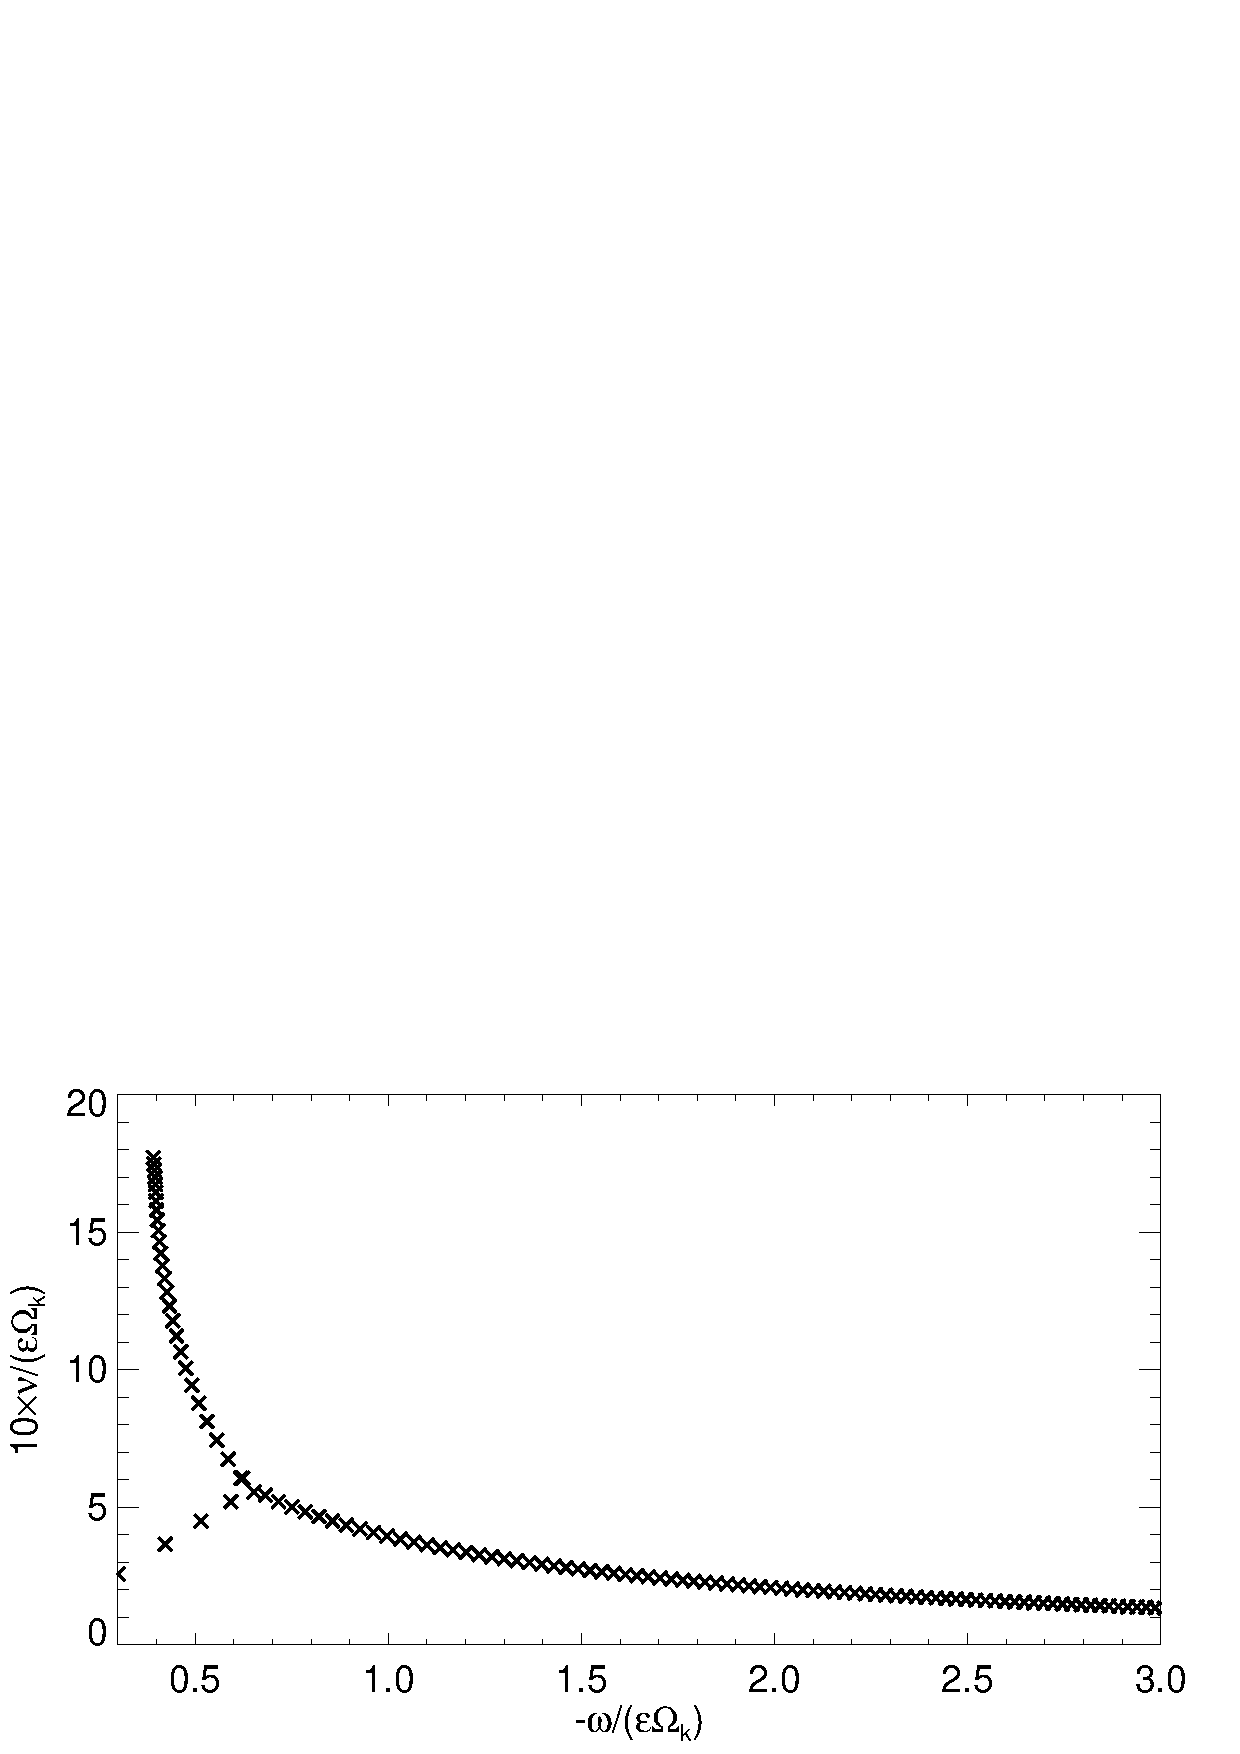
\includegraphics[width=\linewidth]{figures/eigenvalues_iso}
  \caption{Eigenvalues in the low-frequency approximation for the
    vertical shear instability in a vertically isothermal disk evolved
    isothermally ($\gamma=\Gamma=1$). The disk parameters are $q=-1$,
    $p=-1.5$ and $\epsilon=0.1$, while the perturbation radial
    wavenumber is $k_x=200\pi/r$. This is the set up considered in
    \cite{mcnally14}. \label{lowfreq_eigen}
  }
\end{figure}

We plot in Fig. \ref{lowfreq_eigenfunc} the structurally simplest
eigenfunction --- the fundamental corrugation mode corresponding to
the eigenvalue with $\mathrm{min}|\sigma|$. The perturbation $W$ is
roughly proportional to $z$, except close the boundaries where it
flattens because $\delta v_z=dW/dz=0$ is imposed there. 

For $k_x = 200\pi/r$ and $\epsilon = 0.1$, the dimensionless
wavenumber $\hat{k} = k_xH_\mathrm{iso}=20\pi$. Then the expected
growth rate according to Eq. \ref{simple_growth} with $M=1$ is
\begin{align*}
  \nu = 0.2606\epsilon\Omega_k,
\end{align*}
as obtained numerically (Fig. \ref{lowfreq_eigen}). This agreement is
surpsingly good, given that Eq. \ref{simple_growth} assumes the
thin-disk approximation and imposes a different boundary condition to
that in the numerical calculations. 

\begin{figure}
  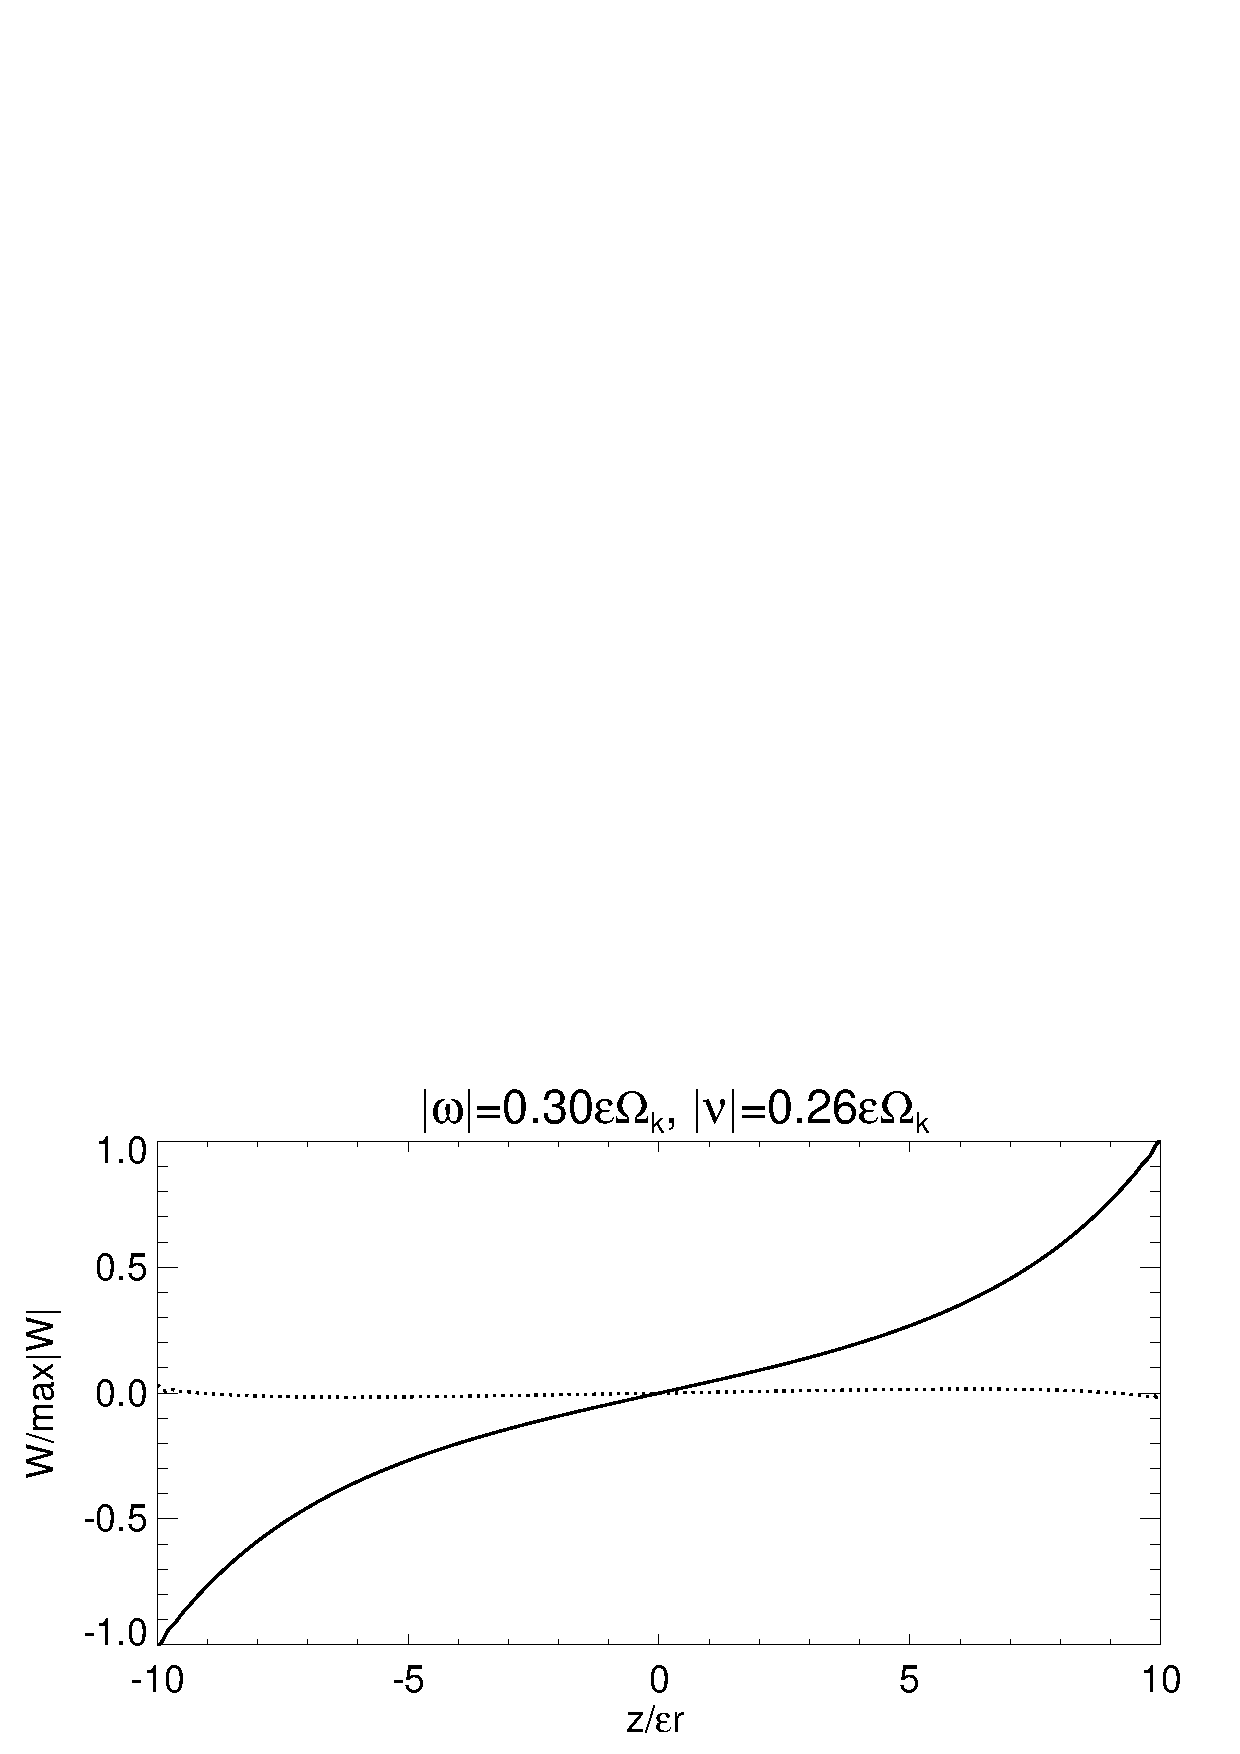
\includegraphics[width=\linewidth]{figures/eigenvector_iso}
  \caption{Eigenfunction of the fundamental corrugation mode,
    corresponding to the 
    bottom-left eigenvalue displayed in Fig. \ref{lowfreq_eigen}. The
    solid and dashed lines are $\real W$ and $\imag W$, respectively. 
    \label{lowfreq_eigenfunc}
  }
\end{figure}

\subsubsection{Influence of vertical boundaries}
